\begin{frame}
\frametitle{Adding explainability with Shapley values}
\begin{columns}
    \begin{column}{0.57\textwidth}
        \begin{itemize}
            \item Shapley values may be used across all model types including deep learning models.
            \item They show the influence of individual data features (including image pixels) and the extent and direction of the influence of that feature.
            \item In the figures red pixels or bars show factors that increase model output value, and blue pixels or bars show factors that reduce model output value.
        \end{itemize}
    \end{column}
    \begin{column}{0.4\textwidth}
        \begin{center}
        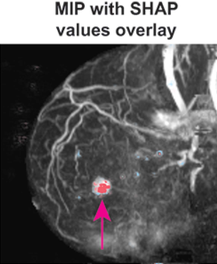
\includegraphics[width=0.6\textwidth]{./misc_images/shap1.png}
        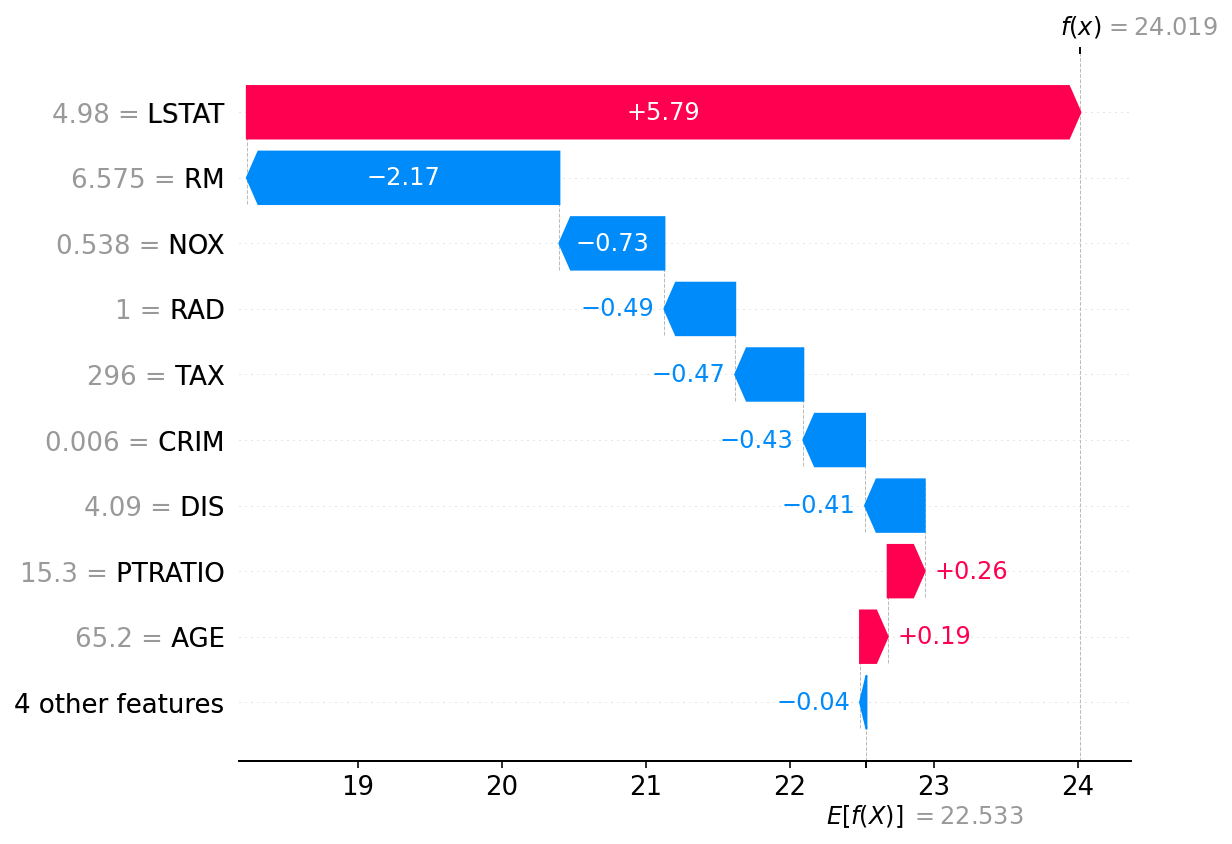
\includegraphics[width=1\textwidth]{./misc_images/shap2.png}
        \end{center}
    \end{column}
\end{columns}
\end{frame}
